%===============================================================================
% $Id: ifacconf.tex 19 2011-10-27 09:32:13Z jpuente $  
% Template for IFAC meeting papers
% Copyright (c) 2007-2008 International Federation of Automatic Control
%===============================================================================
\documentclass{ifacconf}

\usepackage{graphicx}      % include this line if your document contains figures
\usepackage{natbib}        % required for bibliography


\usepackage[T1]{fontenc}
\usepackage[utf8]{inputenc}

% source code listing
\usepackage{listings}
%\usepackage{minted} % some extra configuration an libraries would be necessary


% Sweave Config
 
%results=verbatim, echo=TRUE

%% Sweave

%% SweaveListingUtils
\RequirePackage{fancyvrb}
\RequirePackage{listings}
% %%% important : keep the following comment in
% %%% (see https://mailman.stat.ethz.ch/pipermail/r-help/2009-July/204747.html)
%
% this comment persuades Sweave not to insert \usepackage{Sweave}
%
% -------------------------------------------------------------------------------

% -------------------------------------------------------------------------------


%------------------------------------------------------------------------------%
%Preparations for Sweave and Listings
%------------------------------------------------------------------------------%
%
\RequirePackage{color}
\definecolor{Rcolor}{rgb}{0, 0.5, 0.5}
\definecolor{RRecomdcolor}{rgb}{0, 0.6, 0.4}
\definecolor{Rbcolor}{rgb}{0, 0.6, 0.6}
\definecolor{Routcolor}{rgb}{0.461, 0.039, 0.102}
\definecolor{Rcommentcolor}{rgb}{0.101, 0.043, 0.432}
%------------------------------------------------------------------------------%
\lstdefinelanguage{Rd}[common]{TeX}%
{moretexcs={acronym,alias,arguments,author,bold,cite,%
          code,command,concept,cr,deqn,describe,%
          description,details,dfn,doctype,dots,%
          dontrun,dontshow,donttest,dQuote,%
          email,emph,enc,encoding,enumerate,env,eqn,%
          examples,file,format,if,ifelse,item,itemize,kbd,keyword,%
          ldots,link,linkS4class,method,name,note,%
          option,out,pkg,preformatted,R,Rdopts,Rdversion,%
          references,S3method,S4method,Sexpr,samp,section,%
          seealso,source,sp,special,sQuote,strong,%
          subsection,synopsis,tab,tabular,testonly,%
          title,url,usage,value,var,verb},
   sensitive=true,%
   morecomment=[l]\%% 2008/9 Peter Ruckdeschel
}[keywords,comments]%%
%------------------------------------------------------------------------------%

%----------------
\lstdefinestyle{RstyleO1}{fancyvrb=true,escapechar=`,extendedchars=false,%
                          language=R,%
                          basicstyle={\color{Rcolor}\small},%
                          keywordstyle={\bf\color{Rcolor}},%
                          commentstyle={\color{Rcommentcolor}\ttfamily\itshape},%
                          literate={"}{\texttt{"}}1{<-}{{$\leftarrow$}}2{<<-}{{$\twoheadleftarrow$}}2{~}{{$\sim$}}1{<=}{{$\leq$}}2{>=}{{$\geq$}}2{^}{{$\scriptstyle\wedge$}}1,%
                          alsoother={$},%
                          alsoletter={.<-},%
                          otherkeywords={!,!=,~,$,*,\&,\%/\%,\%*\%,\%\%,<-,<<-,/},%
                          escapeinside={(*}{*)}}%
%----------------
\lstdefinestyle{Rstyle}{style=RstyleO1}

%----------------
\lstdefinestyle{Rdstyle}{fancyvrb=true,language=Rd,keywordstyle={\bf},%
                         basicstyle={\color{black}\footnotesize},%
                         commentstyle={\ttfamily\itshape},%
                         alsolanguage=R}%
%----------------
%------------------------------------------------------------------------------%
\global\def\Rlstset{\lstset{style=Rstyle}}%
\global\def\Rdlstset{\lstset{style=Rdstyle}}%
%------------------------------------------------------------------------------%
\global\def\Rinlstset{\lstset{style=Rinstyle}}%
\global\def\Routlstset{\lstset{style=Routstyle}}%
\global\def\Rcodelstset{\lstset{style=Rcodestyle}}%
%------------------------------------------------------------------------------%
\Rlstset
%------------------------------------------------------------------------------%
%copying relevant parts of Sweave.sty
%------------------------------------------------------------------------------%
%
\RequirePackage{graphicx,fancyvrb}%
\IfFileExists{upquote.sty}{\RequirePackage{upquote}}{}%

\RequirePackage{ifthen}%
\newboolean{Sweave@gin}%
\setboolean{Sweave@gin}{true}%
\setkeys{Gin}{width=0.8\textwidth}%
\newboolean{Sweave@ae}
\setboolean{Sweave@ae}{true}%
\RequirePackage[T1]{fontenc}
\RequirePackage{ae}
%
\newenvironment{Schunk}{}{}

\newcommand{\Sconcordance}[1]{% 
\ifx\pdfoutput\undefined% 
\csname newcount\endcsname\pdfoutput\fi% 
\ifcase\pdfoutput\special{#1}% 
\else\immediate\pdfobj{#1}\fi} 

%------------------------------------------------------------------------------%
% ---- end of parts of Sweave.sty
%------------------------------------------------------------------------------%
%
% ---- input 
\lstdefinestyle{RinstyleO}{style=Rstyle,fancyvrb=true,%
                           basicstyle=\color{Rcolor}\small,%
                           frame=trbl,%
                           frameround=ffff,%
                           backgroundcolor=\color{white},%
                           numbers=left,%
                           numberstyle=\tiny,%
                           stepnumber=1,%
                           numbersep=7pt,%
                           breaklines=TRUE}%
\lstdefinestyle{Rinstyle}{style=RinstyleO}
\lstnewenvironment{Sinput}{\Rinlstset}{\Rlstset}
%
% ---- output 
\lstdefinestyle{RoutstyleO}{fancyvrb=false,basicstyle=\color{Routcolor}\small,%
                            frame=trbl,%
                            frameround=ffff,%
                            backgroundcolor=\color{gray95},%
                            breaklines=TRUE}%
\lstdefinestyle{Routstyle}{style=RoutstyleO}
\lstnewenvironment{Soutput}{\Routlstset}{\Rlstset}
%
% ---- code 
\lstdefinestyle{RcodestyleO}{style=Rstyle,fancyvrb=true,fontshape=sl,%
                             basicstyle=\color{Rcolor}}%
\lstdefinestyle{Rcodestyle}{style=RcodestyleO}
\lstnewenvironment{Scode}{\Rcodelstset}{\Rlstset}
%
%------------------------------------------------------------------------------%
\let\code\lstinline
\def\Code#1{{\tt\color{Rcolor} #1}}
\def\file#1{{\tt #1}} 
\def\pkg#1{{\tt "#1"}} 
\newcommand{\pkgversion}{{\tt 2.1.4}}
%------------------------------------------------------------------------------%

\lstdefinestyle{RstyleO2}{style=RstyleO1,%
% --------------------------
% Registration of package SweaveListingUtils
% --------------------------
morekeywords={[2]taglist,SweaveListingPreparations,SweaveListingOptions,SweaveListingoptions,SweaveListingMASK,%
setToBeDefinedPkgs,setBaseOrRecommended,readSourceFromRForge,readPkgVersion,lstsetRout,%
lstsetRin,lstsetRd,lstsetRcode,lstsetRall,lstsetR,%
lstsetLanguage,lstset,lstinputSourceFromRForge,lstdefRstyle,isBaseOrRecommended,%
getSweaveListingOption,copySourceFromRForge,changeKeywordstyles%
},%
keywordstyle={[2]{\bf}},%
%
% --------------------------
% Registration of package startupmsg
% --------------------------
morekeywords={[3]TOBEDONE,suppressStartupMessages,startupType,startupPackage,StartupMessage,%
startupMessage,startupEndline,readVersionInformation,readURLInformation,pointertoNEWS,%
onlytypeStartupMessages,NEWS,mystartupMessage,mySMHandler,infoShow,%
buildStartupMessage%
},%
keywordstyle={[3]{\bf}},%
%
% --------------------------
% Registration of package cacheSweave
% --------------------------
morekeywords={[4]setCacheDir,getCacheDir,cacheTangleDriver,cacheSweaveDriver%
},%
keywordstyle={[4]{\bf}},%
%
% --------------------------
% Registration of package stashR
% --------------------------
morekeywords={[5]stashROption,setDir<-,reposVersion<-,reposVersion,dbSync,%
copyDB%
},%
keywordstyle={[5]{\bf}},%
%
% --------------------------
% Registration of package filehash
% --------------------------
morekeywords={[6]with,top,registerFormatDB,push,pop,%
mpush,isEmpty,initS,initQ,filehashOption,%
filehashFormats,dumpObjects,dumpList,dumpImage,dumpEnv,%
dumpDF,dbUnlink,dbReorganize,dbMultiFetch,dbLoad,%
dbList,dbLazyLoad,dbInsert,dbInit,dbFetch,%
dbExists,dbDelete,dbCreate,db2env,createS,%
createQ%
},%
keywordstyle={[6]{\bf}},%
%
% --------------------------
% Registration of package ggplot2
% --------------------------
morekeywords={[7]zeroGrob,ylim,ylab,xlim,xlab,%
wrap_hmisc,widthDetails.zeroGrob,vp_path,vp_name,viewports.grobGrid,%
update_stat_defaults,update_labels,update_geom_defaults,uniquecols,ulevels,%
try_require,trim_infinite_01,trim_infinite,TransSqrt,TransReverse,%
TransProbit,TransPow10,TransLogit,TransLog2,TransLog1p,%
TransLog10,TransLog,TransInverse,TransIdentity,transform_position,%
TransExp,TransDatetime,TransDate,TransAtanh,TransAsn,%
Trans,tr,to_time,TopLevel,to_date,%
time_breaks,theme_update,theme_text,theme_set,theme_segment,%
theme_render,theme_rect,theme_line,theme_grey,theme_gray,%
theme_get,theme_bw,theme_blank,surround_viewports,summary.ggplot,%
summarise_by_x,str.uneval,strip_dots,StatVline,stat_vline,%
StatUnique,stat_unique,StatSummary,stat_summary,StatSum,%
stat_sum,StatSpoke,stat_spoke,StatSmooth,stat_smooth,%
StatQuantile,stat_quantile,StatQq,stat_qq,StatIdentity,%
stat_identity,StatHline,stat_hline,StatFunction,stat_function,%
StatDensity2d,stat_density2d,StatDensity,stat_density,StatContour,%
stat_contour,StatBoxplot,stat_boxplot,StatBinhex,stat_binhex,%
StatBin2d,stat_bin2d,StatBin,stat_bin,StatAbline,%
stat_abline,Stat,stairstep,spacer,should_stop,%
setup_viewports,set_last_plot,set_default_scale,seals,scientific,%
scale_z_discrete,scale_y_sqrt,scale_y_reverse,scale_y_recip,scale_y_probit,%
scale_y_prob,scale_y_pow10,scale_y_pow,scale_y_logit,scale_y_log2,%
scale_y_log1p,scale_y_log10,scale_y_log,scale_y_inverse,scale_y_exp,%
scale_y_discrete,scale_y_datetime,scale_y_date,scale_y_continuous,scale_y_atanh,%
scale_y_asn,scale_x_sqrt,scale_x_reverse,scale_x_recip,scale_x_probit,%
scale_x_prob,scale_x_pow10,scale_x_pow,scale_x_logit,scale_x_log2,%
scale_x_log1p,scale_x_log10,scale_x_log,scale_x_inverse,scale_x_exp,%
scale_x_discrete,scale_x_datetime,scale_x_date,scale_x_continuous,scale_x_atanh,%
scale_x_asn,ScaleSqrt,scales_list,scale_size_manual,scale_size_identity,%
ScaleSizeDiscrete,scale_size_discrete,ScaleSizeContinuous,scale_size_continuous,scale_size,%
scale_shape_manual,scale_shape_identity,ScaleShapeDiscrete,scale_shape_discrete,scale_shape,%
Scales,ScaleReverse,ScaleRecip,ScaleProbit,ScaleProb,%
ScalePow10,ScalePow,ScaleManual,ScaleLogit,ScaleLog2,%
ScaleLog1p,ScaleLog10,ScaleLog,scale_linetype_manual,scale_linetype_identity,%
ScaleLinetypeDiscrete,scale_linetype_discrete,scale_linetype,ScaleInverse,ScaleIdentity,%
ScaleHue,ScaleGrey,ScaleGradientn,ScaleGradient2,ScaleGradient,%
scale_fill_manual,scale_fill_identity,scale_fill_hue,scale_fill_grey,scale_fill_gradientn,%
scale_fill_gradient2,scale_fill_gradient,scale_fill_discrete,scale_fill_continuous,scale_fill_brewer,%
ScaleExp,ScaleDiscretePosition,ScaleDiscrete,scale_discrete,ScaleDatetime,%
ScaleDate,ScaleContinuous,scale_colour_manual,scale_colour_identity,scale_colour_hue,%
scale_colour_grey,scale_colour_gradientn,scale_colour_gradient2,scale_colour_gradient,scale_colour_discrete,%
scale_colour_continuous,scale_colour_brewer,ScaleColour,scale_colour,scale_color_manual,%
scale_color_identity,scale_color_hue,scale_color_grey,scale_color_gradientn,scale_color_gradient2,%
scale_color_gradient,scale_color_discrete,scale_color_continuous,scale_color_brewer,ScaleBrewer,%
ScaleAtanh,ScaleAsn,ScaleArea,scale_area,scale_alpha_identity,%
ScaleAlphaContinuous,scale_alpha_continuous,scale_alpha,Scale,save_examples,%
same_file,safe.call,rweave.matrix,rweave.list,rweave.grobGrid,%
rweave,rowHeights,resolution,rescale,rep.unit2,%
rename_aes,remove_missing,rect_to_poly,rdoc_from_html,rdoc_auto_link,%
rbind.grobGrid,quickplot,qplot,ProbabilityTrans,print.uneval,%
print.theme,print.proto,print.grobGrid,print.ggplot,presidential,%
predictdf.loess,predictdf.locfit,predictdf.glm,predictdf.default,predictdf,%
precision,pprint,PowerTrans,pos_stack,PositionStack,%
position_stack,PositionJitter,position_jitter,PositionIdentity,position_identity,%
PositionFill,position_fill,PositionDodge,position_dodge,Position,%
pos_fill,pos_dodge,plot_theme,plotmatrix,plot_clone,%
plist,percent,parse_unit_spec,panelGrob,opts,%
nice_ramp,muted,munch_data,msleep,mpg,%
movies,missing_colour,midwest,median_hilow,mean_se,%
mean_sdl,mean_cl_normal,mean_cl_boot,max2,map_data,%
make_labels,limits.POSIXlt,limits.POSIXct,limits.numeric,limits.factor,%
limits.Date,limits.character,limits,Layer,layer,%
last_plot,labs,label_value,label_parsed,label_bquote,%
label_both,is.zero,is_position_aes,is.integeric,is.constant,%
is_calculated_aes,invert,interp,interleave.unit,interleave.list,%
interleave.default,interleave,html_template_create_all,html_template_create,html_template,%
html_linked_list,html_index_create,html_index,html_autolink_index,html_auto_link,%
hexGrob,hexBin,heightDetails.zeroGrob,guide_legends_box,guide_legends,%
guide_grid,guide_axis,gTree.grobGrid,grobY.absoluteGrob,grobX.absoluteGrob,%
grobWidth.zeroGrob,grobWidth.absoluteGrob,grobs.grobGrid,grobRowHeight,grobRow,%
grobMatrix,grobHeight.zeroGrob,grobHeight.absoluteGrob,grobGrid,grobColWidth,%
grobCol,gridLayout,grid.draw.grobGrid,grid.draw.absoluteGrob,ggstructure,%
ggstrip,ggsave,ggplotGrob,ggplot.default,ggplot.data.frame,%
ggplot_build,ggplot,ggpcp,ggorder,ggopt,%
ggname,ggmissing,ggfluctuation,ggdist,gg_apply,%
get_rev,GeomVline,geom_vline,GeomTile,geom_tile,%
GeomText,geom_text,GeomStep,geom_step,GeomSmooth,%
geom_smooth,GeomSegment,geom_segment,GeomRug,geom_rug,%
GeomRibbon,geom_ribbon,GeomRect,geom_rect,GeomQuantile,%
geom_quantile,GeomPolygon,geom_polygon,GeomPointrange,geom_pointrange,%
GeomPoint,geom_point,GeomPath,geom_path,GeomLinerange,%
geom_linerange,GeomLine,geom_line,GeomJitter,geom_jitter,%
GeomHline,geom_hline,GeomHistogram,geom_histogram,GeomHex,%
geom_hex,GeomFreqpoly,geom_freqpoly,GeomErrorbarh,geom_errorbarh,%
GeomErrorbar,geom_errorbar,GeomDensity2d,geom_density2d,GeomDensity,%
geom_density,GeomCrossbar,geom_crossbar,GeomContour,geom_contour,%
GeomBoxplot,geom_boxplot,GeomBlank,geom_blank,GeomBin2d,%
geom_bin2d,GeomBar,geom_bar,GeomArea,geom_area,%
GeomAbline,geom_abline,Geom,geditGrob,fullseq_time,%
fullseq_date,fullseq,fortify.SpatialPolygonsDataFrame,fortify.SpatialPolygons,fortify.SpatialLinesDataFrame,%
fortify.Polygons,fortify.Polygon,fortify.NULL,fortify.map,fortify.lm,%
fortify.Lines,fortify.Line,fortify.default,fortify.data.frame,fortify,%
force_matrix,floor_time,floor_date,firstUpper,FacetWrap,%
facet_wrap,FacetGrid,facet_grid,Facet,expand_range,%
expand_limits,equal_dims,economics,drawDetails.zeroGrob,dollar,%
dist_polar,dist_euclidean,dist_central_angle,discrete_range,dir_diff,%
dim.grobGrid,digest.proto,digest.ggplot,diamonds,date_breaks,%
cweave.matrix,cweave.list,cweave.grobGrid,cweave,cut_number,%
cut_interval,cunion,CoordTrans,coord_trans,CoordPolar,%
coord_polar,CoordMap,coord_map,CoordFlip,coord_flip,%
CoordFixed,coord_fixed,coord_equal,CoordCartesian,coord_cartesian,%
Coord,compute_intercept,compare_img,comma,colWidths,%
collide,col2hcl,clist,check_required_aesthetics,check_breaks_and_labels,%
ceiling_time,ceiling_date,cbind.grobGrid,build_legend_data,build_legend,%
breaks,borders,bolus.proto,bolus.ggplot,bolus,%
bin,assign_viewports,as.list.unit,as.character.uneval,annotate,%
alpha,all_rdoc_pages_create,all_html_pages_create,all_examples_run,aes_to_scale,%
aes_string,aesdefaults,aes_all,aes,add_missing_levels,%
add_group,accessors_print,absoluteGrob%
},%
keywordstyle={[7]{\bf}},%
%
% --------------------------
% Registration of package grid [recommended or base] 
% --------------------------
morekeywords={[8]yDetails,yaxisGrob,xsplinePoints,xsplineGrob,xDetails,%
xaxisGrob,widthDetails,vpTree,vpStack,vpPath,%
vpList,viewport.transform,viewport.layout,viewport,valid.just,%
validDetails,upViewport,unit.rep,unit.pmin,unit.pmax,%
unit.length,unit.c,unit,textGrob,stringWidth,%
stringHeight,showViewport,showGrob,setGrob,setChildren,%
segmentsGrob,seekViewport,roundrectGrob,removeGrob,rectGrob,%
rasterGrob,pushViewport,push.viewport,preDrawDetails,postDrawDetails,%
popViewport,pop.viewport,polylineGrob,polygonGrob,pointsGrob,%
plotViewport,placeGrob,pathListing,pathGrob,packGrob,%
nullGrob,nestedListing,moveToGrob,lineToGrob,linesGrob,%
layout.widths,layout.torture,layoutRegion,layout.heights,is.unit,%
is.grob,heightDetails,gTree,grobY,grobX,%
grobWidth,grobTree,grobPathListing,grobName,grobHeight,%
grob,grid.yaxis,grid.xspline,grid.xaxis,grid.text,%
grid.strip,grid.show.viewport,grid.show.layout,grid.set,grid.segments,%
grid.roundrect,grid.remove,grid.refresh,grid.rect,grid.record,%
grid.raster,grid.prompt,grid.pretty,grid.polyline,grid.polygon,%
grid.points,grid.plot.and.legend,grid.place,grid.path,grid.panel,%
grid.pack,grid.null,grid.newpage,grid.multipanel,grid.move.to,%
grid.ls,grid.locator,grid.line.to,grid.lines,grid.legend,%
grid.layout,grid.grob,grid.grill,grid.gremove,grid.grabExpr,%
grid.grab,grid.gget,grid.get,grid.gedit,grid.function,%
grid.frame,grid.edit,grid.draw,grid.display.list,grid.curve,%
grid.copy,grid.convertY,grid.convertX,grid.convertWidth,grid.convertHeight,%
grid.convert,grid.collection,grid.clip,grid.circle,grid.cap,%
grid.arrows,grid.add,grid.abline,gPath,gpar,%
gList,getNames,getGrob,get.gpar,gEditList,%
gEdit,functionGrob,frameGrob,engine.display.list,editGrob,%
editDetails,drawDetails,draw.details,downViewport,dataViewport,%
curveGrob,current.vpTree,current.vpPath,current.viewport,current.transform,%
convertY,convertX,convertWidth,convertUnit,convertNative,%
convertHeight,clipGrob,circleGrob,childNames,arrowsGrob,%
arrow,arcCurvature,applyEdits,applyEdit,addGrob,%
absolute.size%
},%
keywordstyle={[8]{\bf\color{RRecomdcolor}}},%
%
% --------------------------
% Registration of package reshape
% --------------------------
morekeywords={[9]updatelist,untable,uniquedefault,tips,tidystamp,%
strip.dups,str.cast_matrix,str.cast_df,stamp,sparseby,%
sort_df,smiths,rrownames<-,rrownames,round_any,%
reshape1,rescaler.matrix,rescaler.default,rescaler.data.frame,rescaler,%
rename,recast,rdimnames<-,rdimnames,rcolnames<-,%
rcolnames,print.cast_matrix,print.cast_df,prettyprint,nulldefault,%
nested.by,namerows,merge_recurse,merge_all,melt.table,%
melt.matrix,melt.list,melt.default,melt.data.frame,melt_check,%
melt.cast_matrix,melt.cast_df,melt.array,melt,margin.vars,%
guess_value,funstofun,french_fries,expand.grid.df,dim_names,%
condense.df,condense,compute.margins,combine_factor,colsplit.factor,%
colsplit.character,colsplit,clean.vars,check_formula,cast_parse_formula,%
cast_matrix,cast,as.matrix.cast_matrix,as.matrix.cast_df,as.data.frame.cast_matrix,%
as.data.frame.cast_df,all.vars.character,add.missing.levels,add.all.combinations%
},%
keywordstyle={[9]{\bf}},%
%
% --------------------------
% Registration of package plyr
% --------------------------
morekeywords={[10]vaggregate,unrowname,try_default,tryapply,true,%
summarize,summarise,strip_splits,split_labels,splat,%
r_ply,round_any,rlply,rename,rdply,%
rbind.fill.matrix,rbind.fill,raply,quickdf,progress_win,%
progress_tk,progress_text,progress_none,ozone,numcolwise,%
mutate,m_ply,mlply,mdply,match_df,%
maply,l_ply,llply,liply,ldply,%
laply,join.keys,join,is.quoted,isplit2,%
is.formula,is.discrete,idata.frame,id,failwith,%
eval.quoted,empty,each,d_ply,dlply,%
desc,defaults,ddply,daply,create_progress_bar,%
compact,colwise,catcolwise,baseball,as.quoted,%
arrange,a_ply,amv_dimnames,alply,adply,%
aaply%
},%
keywordstyle={[10]{\bf}},%
%
% --------------------------
% Registration of package stringr
% --------------------------
morekeywords={[11]word,str_wrap,str_trim,str_sub<-,str_sub,%
str_split_fixed,str_split,str_replace_all,str_replace,str_pad,%
str_match_all,str_match,str_locate_all,str_locate,str_length,%
str_extract_all,str_extract,str_dup,str_detect,str_count,%
str_c,perl,invert_match,ignore.case,fixed%
},%
keywordstyle={[11]{\bf}},%
%
% --------------------------
% Registration of package sqldf
% --------------------------
morekeywords={[12]sqldf,read.csv.sql,read.csv2.sql%
},%
keywordstyle={[12]{\bf}},%
%
% --------------------------
% Registration of package chron
% --------------------------
morekeywords={[13]year.strict,years,year.expand,times,seq.dates,%
seconds,month.day.year,minutes,leap.year,is.weekend,%
is.holiday,is.chron,hours,days,day.of.week,%
dates,chron,as.chron%
},%
keywordstyle={[13]{\bf}},%
%
% --------------------------
% Registration of package gsubfn
% --------------------------
morekeywords={[14]strapply1,strapply,paste0,ostrapply,matrixfn,%
match.funfn,gsubfn,fn,eval.with.vis,cat0,%
as.function.formula%
},%
keywordstyle={[14]{\bf}},%
%
% --------------------------
% Registration of package proto
% --------------------------
morekeywords={[15]str.proto,proto,print.instantiatedProtoMethod,name.proto,is.proto,%
isnot.function,graph.proto,as.proto.proto,as.proto.list,as.proto.environment,%
as.proto%
},%
keywordstyle={[15]{\bf}},%
%
% --------------------------
% Registration of package DBI
% --------------------------
morekeywords={[16]SQLKeywords,print.list.pairs,make.db.names.default,make.db.names,isSQLKeyword.default,%
isSQLKeyword,fetch,dbWriteTable,dbUnloadDriver,dbSetDataMappings,%
dbSendQuery,dbRollback,dbRemoveTable,dbReadTable,dbListTables,%
dbListResults,dbListFields,dbListConnections,dbHasCompleted,dbGetStatement,%
dbGetRowsAffected,dbGetRowCount,dbGetQuery,dbGetInfo,dbGetException,%
dbGetDBIVersion,dbExistsTable,dbDriver,dbDisconnect,dbDataType.default,%
dbDataType,dbConnect,dbCommit,dbColumnInfo,dbClearResult,%
dbCallProc%
},%
keywordstyle={[16]{\bf}},%
%
% --------------------------
% Registration of package xtable
% --------------------------
morekeywords={[17]xtable,label<-,label,display<-,display,%
digits<-,digits,caption<-,caption,align<-,%
align%
},%
keywordstyle={[17]{\bf}},%
%
% --------------------------
% Registration of package log4r
% --------------------------
morekeywords={[18]warn,verbosity,logformat.logger,logformat<-.logger,logformat<-,%
logformat,logfile.logger,logfile<-.logger,logfile<-,logfile,%
level.logger,level<-.logger,level<-,level,info,%
fatal,error,create.logger%
},%
keywordstyle={[18]{\bf}},%
%
% --------------------------
% Registration of package testthat
% --------------------------
morekeywords={[19]watch,throws_error,test_that,test_package,test_file,%
test_dir,takes_less_than,SummaryReporter,StopReporter,source_dir,%
shows_message,prints_text,MinimalReporter,matches,library_if_available,%
is_true,is_identical_to,is_false,is_equivalent_to,is_a,%
gives_warning,expect_warning,expect_true,expect_that,expect_output,%
expect_message,expect_match,expect_is,expect_identical,expect_false,%
expect_error,expect_equivalent,expect_equal,expectation,equals,%
context,colourise,auto_test_package,auto_test%
},%
keywordstyle={[19]{\bf}},%
%
% --------------------------
% Registration of package stats [recommended or base] 
% --------------------------
morekeywords={[20]xtabs,write.ftable,window<-,wilcox.test,weighted.residuals,%
weighted.mean,vcov,var.test,varimax,variable.names,%
update.formula,update.default,TukeyHSD.aov,TukeyHSD,t.test,%
ts.union,tsSmooth,ts.plot,tsp<-,ts.intersect,%
tsdiag,toeplitz,terms.terms,terms.formula,terms.default,%
terms.aovlist,termplot,supsmu,summary.stepfun,summary.mlm,%
summary.manova,summary.lm,summary.infl,summary.glm,summary.aovlist,%
summary.aov,StructTS,stl,stepfun,stat.anova,%
SSweibull,SSmicmen,SSlogis,SSgompertz,SSfpl,%
SSfol,SSD,SSbiexp,SSasympOrig,SSasympOff,%
SSasymp,splinefunH,spectrum,spec.taper,spec.pgram,%
spec.ar,sortedXyData,smooth.spline,smoothEnds,smooth,%
simulate,shapiro.test,setNames,selfStart,se.contrast,%
screeplot,scatter.smooth,runmed,rstudent.lm,rstudent.glm,%
rstandard.lm,rstandard.glm,rmultinom,residuals.lm,residuals.glm,%
residuals.default,reshapeWide,reshapeLong,reshape,reorder,%
rect.hclust,read.ftable,r2dtable,quasipoisson,quasibinomial,%
quantile.default,quade.test,qqnorm.default,qbirthday,prop.trend.test,%
prop.test,promax,print.ts,print.terms,print.logLik,%
print.lm,print.integrate,print.infl,print.glm,print.ftable,%
print.formula,print.family,print.density,printCoefmat,print.coefmat,%
print.anova,princomp,predict.poly,predict.mlm,predict.lm,%
predict.glm,prcomp,PP.test,ppr,power.t.test,%
power.prop.test,power.anova.test,polym,poisson.test,plot.TukeyHSD,%
plot.ts,plot.stepfun,plot.spec.phase,plot.spec.coherency,plot.spec,%
plot.mlm,plot.lm,plot.ecdf,plot.density,plclust,%
pbirthday,pairwise.wilcox.test,pairwise.t.test,pairwise.table,pairwise.prop.test,%
p.adjust.methods,p.adjust,pacf,order.dendrogram,oneway.test,%
numericDeriv,nobs,NLSstRtAsymptote,NLSstLfAsymptote,NLSstClosestX,%
NLSstAsymptotic,nls.control,nls,nlminb,naresid,%
naprint,napredict,na.pass,na.omit,na.fail,%
na.exclude,na.contiguous,na.action,mood.test,monthplot,%
model.weights,model.tables,model.response,model.offset,model.matrix.lm,%
model.matrix.default,model.matrix,model.frame.lm,model.frame.glm,model.frame.default,%
model.frame.aovlist,model.frame,model.extract,medpolish,median.default,%
mcnemar.test,mauchly.test,mauchley.test,mantelhaen.test,manova,%
makepredictcall,make.link,makeARIMA,ls.print,ls.diag,%
logLik,loess.smooth,loess.control,loess,loadings,%
lm.wfit.null,lm.wfit,lm.influence,lm.fit.null,lm.fit,%
lines.ts,line,lag.plot,lag,ks.test,%
ksmooth,kruskal.test,knots,kmeans,kernel,%
kernapply,KalmanSmooth,KalmanRun,KalmanLike,KalmanForecast,%
is.tskernel,is.ts,is.stepfun,isoreg,is.mts,%
is.leaf,is.empty.model,inverse.gaussian,interaction.plot,integrate,%
influence.measures,HoltWinters,heatmap,hclust,hatvalues.lm,%
hatvalues,glm.fit.null,glm.fit,glm.control,getInitial,%
getCall,get_all_vars,friedman.test,fligner.test,fitted.values,%
fisher.test,filter,factor.scope,factanal,expand.model.frame,%
estVar,embed,eff.aovlist,ecdf,dummy.coef,%
drop.terms,drop.scope,dmultinom,dist,diff.ts,%
diffinv,df.residual,df.kernel,dfbeta,deriv.formula,%
deriv.default,deriv3.formula,deriv3.default,deriv3,density.default,%
dendrapply,delete.response,decompose,cutree,cpgram,%
cov.wt,cov2cor,cor.test,cophenetic,cooks.distance,%
contr.treatment,contr.sum,contr.SAS,contr.poly,contr.helmert,%
contrasts<-,constrOptim,confint.default,confint,complete.cases,%
cmdscale,clearNames,chisq.test,ccf,case.names,%
cancor,bw.ucv,bw.SJ,bw.nrd0,bw.nrd,%
bw.bcv,Box.test,biplot,binom.test,BIC,%
bartlett.test,bandwidth.kernel,as.ts,as.stepfun,asOneSidedFormula,%
as.hclust,as.formula,as.dist,as.dendrogram,ar.yw,%
ar.ols,ar.mle,ARMAtoMA,ARMAacf,arima.sim,%
arima0.diag,arima0,arima,ar.burg,ar,%
ansari.test,anova.mlm,anova.lmlist,anova.lm,anovalist.lm,%
anova.glmlist,anova.glm,AIC,aggregate.ts,aggregate.default,%
aggregate.data.frame,add.scope,addmargins,acf2AR,acf%
},%
keywordstyle={[20]{\bf\color{RRecomdcolor}}},%
%
% --------------------------
% Registration of package graphics [recommended or base] 
% --------------------------
morekeywords={[21]xspline,text.default,stripchart,strheight,split.screen,%
spineplot,smoothScatter,rasterImage,polypath,points.default,%
plot.xy,plot.window,plot.new,plot.function,plot.design,%
plot.default,pie,panel.smooth,pairs.default,lines.default,%
layout.show,image.default,hist.default,grconvertY,grconvertX,%
fourfoldplot,filled.contour,erase.screen,dotchart,contour.default,%
co.intervals,close.screen,clip,cdplot,boxplot.matrix,%
boxplot.default,barplot.default,axTicks,axis.POSIXct,axis.Date,%
Axis,assocplot%
},%
keywordstyle={[21]{\bf\color{RRecomdcolor}}},%
%
% --------------------------
% Registration of package grDevices [recommended or base] 
% --------------------------
morekeywords={[22]xyz.coords,xyTable,xy.coords,xfig,X11.options,%
X11Fonts,X11Font,Type1Font,trans3d,topo.colors,%
tiff,terrain.colors,svg,setPS,setGraphicsEventHandlers,%
setGraphicsEventEnv,setEPS,savePlot,rgb2hsv,replayPlot,%
recordPlot,recordGraphics,quartz.options,quartzFonts,quartzFont,%
quartz,ps.options,postscriptFonts,postscriptFont,png,%
pdf.options,pdfFonts,pdf,nclass.Sturges,nclass.scott,%
nclass.FD,n2mfrow,make.rgb,jpeg,is.raster,%
Hershey,heat.colors,hcl,grey.colors,gray.colors,%
graphics.off,getGraphicsEventEnv,getGraphicsEvent,extendrange,embedFonts,%
dev.size,dev.set,dev.print,dev.prev,dev.off,%
dev.next,dev.new,dev.list,dev.interactive,deviceIsInteractive,%
dev.hold,dev.flush,dev.cur,dev.copy2pdf,dev.copy2eps,%
dev.copy,dev.control,dev.capture,dev.capabilities,devAskNewPage,%
densCols,convertColor,contourLines,colorspaces,colorRampPalette,%
colorRamp,colorConverter,col2rgb,cm.colors,CIDFont,%
check.options,cairo_ps,cairo_pdf,boxplot.stats,bmp,%
blues9,bitmap,axisTicks,as.raster,as.graphicsAnnot,%
adjustcolor%
},%
keywordstyle={[22]{\bf\color{RRecomdcolor}}},%
%
% --------------------------
% Registration of package utils [recommended or base] 
% --------------------------
morekeywords={[23]zip.file.extract,wsbrowser,write.table,write.socket,write.csv2,%
write.csv,vignette,View,url.show,URLencode,%
URLdecode,upgrade,update.packageStatus,update.packages,unzip,%
untar,unstack,type.convert,txtProgressBar,toLatex,%
toBibtex,timestamp,tar,tail.matrix,tail,%
SweaveSyntConv,SweaveSyntaxNoweb,SweaveSyntaxLatex,SweaveHooks,Sweave,%
summaryRprof,strOptions,str,Stangle,stack,%
setTxtProgressBar,setRepositories,setBreakpoint,sessionInfo,select.list,%
savehistory,RweaveTryStop,RweaveLatexWritedoc,RweaveLatexSetup,RweaveLatexOptions,%
RweaveLatexFinish,RweaveLatex,RweaveEvalWithOpt,RweaveChunkPrefix,RtangleWritedoc,%
RtangleSetup,Rtangle,rtags,RSiteSearch,RShowDoc,%
Rprofmem,Rprof,removeSource,remove.packages,relist,%
recover,read.table,read.socket,read.fwf,read.fortran,%
read.DIF,read.delim2,read.delim,read.csv2,read.csv,%
readCitationFile,rc.status,rc.settings,rc.options,rc.getOption,%
promptPackage,promptData,personList,person,packageVersion,%
packageStatus,package.skeleton,packageDescription,package.contents,old.packages,%
object.size,nsl,news,new.packages,modifyList,%
mirror2html,memory.size,memory.limit,make.socket,makeRweaveLatexCodeRunner,%
make.packages.html,maintainer,ls.str,lsf.str,localeToCharset,%
loadhistory,limitedLabels,is.relistable,install.packages,installed.packages,%
history,help.start,help.search,help.request,head.matrix,%
head,glob2rx,getTxtProgressBar,getSrcref,getSrcLocation,%
getSrcFilename,getSrcDirectory,getS3method,getFromNamespace,getCRANmirrors,%
getAnywhere,formatUL,formatOL,flush.console,fixInNamespace,%
findLineNum,file_test,file.edit,dump.frames,download.packages,%
download.file,de.setup,de.restore,de.ncols,data.entry,%
create.post,CRAN.packages,count.fields,contrib.url,compareVersion,%
combn,close.socket,citHeader,citFooter,citEntry,%
citation,chooseCRANmirror,chooseBioCmirror,checkCRAN,capture.output,%
bug.report,browseVignettes,browseURL,browseEnv,bibentry,%
available.packages,assignInNamespace,as.roman,as.relistable,as.personList,%
as.person,aspell_write_personal_dictionary_file,aspell_package_vignettes,aspell_package_Rd_files,aspell,%
argsAnywhere,aregexec,alarm,adist%
},%
keywordstyle={[23]{\bf\color{RRecomdcolor}}},%
%
% --------------------------
% Registration of package datasets [recommended or base] 
% --------------------------
morekeywords={[24]WWWusage,WorldPhones,women,warpbreaks,volcano,%
VADeaths,uspop,USPersonalExpenditure,USJudgeRatings,USArrests,%
USAccDeaths,UKgas,UKDriverDeaths,UCBAdmissions,trees,%
treering,ToothGrowth,Titanic,Theoph,swiss,%
sunspot.year,sunspots,sunspot.month,state.x77,state.region,%
state.name,state.division,state.center,state.area,state.abb,%
stack.x,stack.loss,stackloss,sleep,Seatbelts,%
rock,rivers,randu,quakes,Puromycin,%
pressure,presidents,precip,PlantGrowth,OrchardSprays,%
Orange,occupationalStatus,nottem,Nile,nhtemp,%
mtcars,morley,mdeaths,lynx,longley,%
Loblolly,LifeCycleSavings,lh,ldeaths,LakeHuron,%
JohnsonJohnson,islands,iris3,iris,InsectSprays,%
infert,Indometh,Harman74.cor,Harman23.cor,HairEyeColor,%
freeny.y,freeny.x,freeny,Formaldehyde,fdeaths,%
faithful,EuStockMarkets,eurodist,euro.cross,euro,%
esoph,DNase,discoveries,crimtab,CO2,%
co2,chickwts,ChickWeight,cars,BOD,%
BJsales.lead,BJsales,beaver2,beaver1,austres,%
attitude,attenu,anscombe,airquality,AirPassengers,%
airmiles,ability.cov%
},%
keywordstyle={[24]{\bf\color{RRecomdcolor}}},%
%
% --------------------------
% Registration of package methods [recommended or base] 
% --------------------------
morekeywords={[25]validSlotNames,validObject,unRematchDefinition,trySilent,tryNew,%
traceOn,traceOff,testVirtual,testInheritedMethods,superClassDepth,%
Summary,substituteFunctionArgs,substituteDirect,slotsFromS3,slotNames,%
slot<-,slot,sigToEnv,SignatureMethod,signature,%
showMlist,showMethods,showExtends,showDefault,showClass,%
setValidity,setReplaceMethod,setRefClass,setPrimitiveMethods,setPackageName,%
setOldClass,setMethod,setIs,setGroupGeneric,setGenericImplicit,%
setGeneric,setDataPart,setClassUnion,setClass,setAs,%
sessionData,selectSuperClasses,selectMethod,seemsS4Object,sealClass,%
S3Part<-,S3Part,S3Class<-,S3Class,resetGeneric,%
resetClass,requireMethods,representation,removeMethodsObject,removeMethods,%
removeMethod,removeGeneric,removeClass,rematchDefinition,registerImplicitGenerics,%
reconcilePropertiesAndPrototype,rbind2,Quote,prototype,promptMethods,%
promptClass,prohibitGeneric,possibleExtends,packageSlot<-,packageSlot,%
newEmptyObject,newClassRepresentation,newBasic,multipleClasses,mlistMetaName,%
missingArg,methodsPackageMetaName,MethodsListSelect,MethodsList,method.skeleton,%
methodSignatureMatrix,MethodAddCoerce,metaNameUndo,mergeMethods,Math2,%
matchSignature,makeStandardGeneric,makePrototypeFromClassDef,makeMethodsList,makeGeneric,%
makeExtends,makeClassRepresentation,Logic,loadMethod,listFromMlist,%
listFromMethods,linearizeMlist,languageEl<-,languageEl,isXS3Class,%
isVirtualClass,isSealedMethod,isSealedClass,isGroup,isGrammarSymbol,%
isGeneric,isClassUnion,isClassDef,isClass,insertSource,%
insertMethod,initRefFields,initialize,initFieldArgs,inheritedSlotNames,%
implicitGeneric,hasMethods,hasMethod,hasArg,getVirtual,%
getValidity,getSubclasses,getSlots,getRefClass,getPrototype,%
getProperties,getPackageName,getMethodsMetaData,getMethodsForDispatch,getMethods,%
getMethod,getGroupMembers,getGroup,getGenerics,getGeneric,%
getFunction,getExtends,getDataPart,getClassPackage,getClassName,%
getClasses,getClassDef,getClass,getAllSuperClasses,getAllMethods,%
getAccess,generic.skeleton,functionBody<-,functionBody,formalArgs,%
fixPre1.8,findUnique,findMethodSignatures,findMethods,findMethod,%
findFunction,findClass,finalDefaultMethod,extends,existsMethod,%
existsFunction,evalSource,emptyMethodsList,empty.dump,elNamed<-,%
elNamed,el<-,el,dumpMethods,dumpMethod,%
doPrimitiveMethod,defaultPrototype,defaultDumpName,conformMethod,Complex,%
completeSubclasses,completeExtends,completeClassDefinition,Compare,coerce<-,%
coerce,className,classMetaName,classLabel,classesToAM,%
checkSlotAssignment,cbind2,canCoerce,callNextMethod,callGeneric,%
cacheMethod,cacheMetaData,cacheGenericsMetaData,body<-,balanceMethodsList,%
assignMethodsMetaData,assignClassDef,asMethodDefinition,as<-,Arith,%
allNames,allGenerics,addNextMethod%
},%
keywordstyle={[25]{\bf\color{RRecomdcolor}}},%
%
% --------------------------
% Registration of package base [recommended or base] 
% --------------------------
morekeywords={[26]xzfile,xtfrm.Surv,xtfrm.POSIXlt,xtfrm.POSIXct,xtfrm.numeric_version,%
xtfrm.factor,xtfrm.difftime,xtfrm.default,xtfrm.Date,xtfrm.AsIs,%
xtfrm,xpdrows.data.frame,xor.octmode,xor.hexmode,write.table0,%
writeLines,write.dcf,writeChar,writeBin,withVisible,%
withRestarts,within.list,within.data.frame,within,with.default,%
withCallingHandlers,with,which.min,which.max,weekdays.POSIXt,%
weekdays.Date,weekdays,version,Vectorize,vapply,%
utf8ToInt,upper.tri,unz,untracemem,unsplit,%
unserialize,unlockBinding,unloadNamespace,unix.time,units.difftime,%
units<-.difftime,units<-,units,unique.POSIXlt,unique.numeric_version,%
unique.matrix,unique.default,unique.data.frame,unique.array,tryCatch,%
trunc.POSIXt,trunc.Date,truncate.connection,truncate,transform.default,%
transform.data.frame,tracingState,tracemem,toupper,toString.default,%
toString,topenv,tolower,textConnectionValue,textConnection,%
testPlatformEquivalence,tempdir,t.default,t.data.frame,tcrossprod,%
taskCallbackManager,T,Sys.which,Sys.unsetenv,Sys.umask,%
Sys.timezone,Sys.time,system.time,system.file,system2,%
sys.status,sys.source,Sys.sleep,Sys.setlocale,Sys.setFileTime,%
Sys.setenv,sys.save.image,Sys.readlink,Sys.putenv,sys.parents,%
sys.parent,sys.on.exit,sys.nframe,Sys.localeconv,sys.load.image,%
Sys.info,Sys.glob,Sys.getpid,Sys.getlocale,Sys.getenv,%
sys.function,sys.frames,sys.frame,Sys.Date,Sys.chmod,%
sys.calls,sys.call,symbol.For,symbol.C,suppressWarnings,%
suppressPackageStartupMessages,suppressMessages,summary.table,summary.srcref,summary.srcfile,%
Summary.POSIXlt,summary.POSIXlt,Summary.POSIXct,summary.POSIXct,Summary.ordered,%
Summary.numeric_version,summary.matrix,Summary.factor,summary.factor,Summary.difftime,%
summary.default,Summary.Date,summary.Date,Summary.data.frame,summary.data.frame,%
summary.connection,substring<-,substr<-,subset.matrix,subset.default,%
subset.data.frame,strwrap,strtrim,strtoi,strptime,%
strftime,storage.mode<-,storage.mode,stopifnot,stdout,%
stdin,stderr,standardGeneric,srcref,srcfilecopy,%
srcfilealias,srcfile,sQuote,sprintf,split.POSIXct,%
split.default,split<-.default,split.Date,split.data.frame,split<-.data.frame,%
split<-,source.url,sort.POSIXlt,sort.list,sort.int,%
sort.default,solve.qr,solve.default,socketSelect,socketConnection,%
slice.index,sink.number,simplify2array,simpleWarning,simpleMessage,%
simpleError,simpleCondition,signalCondition,shQuote,showConnections,%
setTimeLimit,setSessionTimeLimit,set.seed,setNamespaceInfo,setHook,%
setCConverterStatus,serialize,seq.POSIXt,seq_len,seq.int,%
seq.default,seq.Date,seq_along,seek.connection,seek,%
scan.url,scale.default,saveRDS,save.image,sample.int,%
R.version.string,R.Version,R.version,R_system_version,rowSums,%
rowsum.default,rowsum.data.frame,row.names.default,row.names<-.default,row.names.data.frame,%
row.names<-.data.frame,rownames<-,row.names<-,row.names,rowMeans,%
round.POSIXt,round.Date,RNGversion,R.home,rev.default,%
retracemem,restartFormals,restartDescription,requireNamespace,rep.POSIXlt,%
rep.POSIXct,rep.numeric_version,replicate,rep.int,rep.factor,%
rep.Date,removeTaskCallback,removeCConverter,regmatches<-,regmatches,%
registerS3methods,registerS3method,reg.finalizer,regexec,Reduce,%
read.table.url,readRenviron,readRDS,readLines,read.dcf,%
readChar,readBin,rcond,rbind.data.frame,rawToChar,%
rawToBits,rawShift,rawConnectionValue,rawConnection,raw,%
rapply,range.default,quarters.POSIXt,quarters.Date,quarters,%
qr.X,qr.solve,qr.resid,qr.R,qr.qy,%
qr.qty,qr.Q,qr.fitted,qr.default,qr.coef,%
pushBackLength,pushBack,psigamma,prop.table,proc.time,%
print.warnings,print.table,print.summary.table,print.summaryDefault,print.srcref,%
print.srcfile,print.simple.list,print.rle,print.restart,print.proc_time,%
print.POSIXlt,print.POSIXct,print.packageInfo,print.octmode,print.numeric_version,%
print.noquote,printNoClass,print.NativeRoutineList,print.listof,print.libraryIQR,%
print.hexmode,print.function,print.factor,print.DLLRegisteredRoutines,print.DLLInfoList,%
print.DLLInfo,print.difftime,print.default,print.Date,print.data.frame,%
print.connection,print.condition,print.by,print.AsIs,prettyNum,%
pretty.default,pos.to.env,Position,pmin.int,pmax.int,%
pipe,pi,path.package,path.expand,parseNamespaceFile,%
parse.dcf,parent.frame,parent.env<-,parent.env,packBits,%
package_version,packageStartupMessage,packageHasNamespace,packageEvent,package.description,%
Ops.POSIXt,Ops.ordered,Ops.numeric_version,Ops.factor,Ops.difftime,%
Ops.Date,Ops.data.frame,open.srcfilecopy,open.srcfilealias,open.srcfile,%
open.connection,open,on.exit,oldClass<-,oldClass,%
nzchar,numeric_version,normalizePath,norm,ngettext,%
new.env,Negate,names.POSIXlt,names<-.POSIXlt,namespaceImportMethods,%
namespaceImportFrom,namespaceImportClasses,namespaceImport,namespaceExport,names<-,%
mostattributes<-,months.POSIXt,months.Date,months,month.name,%
month.abb,mode<-,mget,message,merge.default,%
merge.data.frame,memory.profile,mem.limits,memDecompress,memCompress,%
mean.POSIXlt,mean.POSIXct,mean.difftime,mean.default,mean.Date,%
mean.data.frame,max.col,mat.or.vec,Math.POSIXt,Math.factor,%
Math.difftime,Math.Date,Math.data.frame,match.fun,match.call,%
match.arg,margin.table,mapply,Map,manglePackageName,%
make.unique,make.names,makeActiveBinding,lower.tri,logb,%
lockEnvironment,lockBinding,loadURL,loadNamespace,loadingNamespaceInfo,%
loadedNamespaces,list.files,list.dirs,list2env,library.dynam.unload,%
library.dynam,lfactorial,levels<-.factor,levels.default,levels<-,%
LETTERS,letters,length.POSIXlt,length<-.factor,length<-,%
lazyLoadDBfetch,lazyLoadDBexec,lazyLoad,La.svd,La.eigen,%
La.chol2inv,La.chol,labels.default,l10n_info,kappa.tri,%
kappa.qr,kappa.lm,kappa.default,julian.POSIXt,julian.Date,%
julian,is.vector,is.unsorted,isTRUE,is.table,%
isSymmetric.matrix,isSymmetric,is.symbol,is.single,isSeekable,%
isS4,isRestart,is.recursive,is.real,is.raw,%
is.R,is.qr,is.primitive,is.pairlist,is.package_version,%
is.ordered,isOpen,ISOdatetime,ISOdate,is.object,%
is.numeric_version,is.numeric.POSIXt,is.numeric.difftime,is.numeric.Date,is.numeric,%
is.null,is.na.POSIXlt,is.na.numeric_version,is.nan,isNamespace,%
is.name,is.na<-.factor,is.na<-.default,is.na.data.frame,is.na<-,%
is.na,is.matrix,is.logical,is.loaded,is.list,%
is.language,is.integer,is.infinite,isIncomplete,is.function,%
is.finite,is.factor,is.expression,is.environment,is.element,%
is.double,isdebugged,is.data.frame,is.complex,is.character,%
is.call,isBaseNamespace,isatty,is.atomic,is.array,%
invokeRestartInteractively,invokeRestart,inverse.rle,intToUtf8,intToBits,%
importIntoEnv,identity,identical,icuSetCollate,iconvlist,%
iconv,gzfile,gzcon,grepRaw,grepl,%
gregexpr,gettextf,gettext,getTaskCallbackNames,getSrcLines,%
getRversion,getNumCConverters,getNativeSymbolInfo,getNamespaceVersion,getNamespaceUsers,%
getNamespaceName,getNamespaceInfo,getNamespaceImports,getNamespaceExports,getNamespace,%
getLoadedDLLs,getHook,getExportedValue,getElement,getDLLRegisteredRoutines.DLLInfo,%
getDLLRegisteredRoutines.character,getDLLRegisteredRoutines,getConnection,getCConverterStatus,getCConverterDescriptions,%
getCallingDLLe,getCallingDLL,getAllConnections,gctorture2,gc.time,%
format.pval,format.POSIXlt,format.POSIXct,format.packageInfo,format.octmode,%
format.numeric_version,format.libraryIQR,format.info,format.hexmode,format.factor,%
formatDL,format.difftime,format.default,format.Date,format.data.frame,%
format.char,format.AsIs,formals<-,force,flush.connection,%
flush,findRestart,findPackageEnv,find.package,findInterval,%
Find,Filter,file.symlink,file.show,file.rename,%
file.remove,file.path,file.link,file.info,file.exists,%
file.create,file.copy,file.choose,file.append,file.access,%
fifo,factorial,F,expm1,expand.grid,%
eval.parent,env.profile,environmentName,environmentIsLocked,environment<-,%
enquote,Encoding<-,Encoding,encodeString,enc2utf8,%
enc2native,emptyenv,eapply,dyn.unload,dyn.load,%
duplicated.POSIXlt,duplicated.numeric_version,duplicated.matrix,duplicated.default,duplicated.data.frame,%
duplicated.array,droplevels.factor,droplevels.data.frame,droplevels,dQuote,%
do.call,dir.create,dimnames.data.frame,dimnames<-.data.frame,dimnames<-,%
dim.data.frame,dim<-,difftime,diff.POSIXt,diff.default,%
diff.Date,diag<-,determinant.matrix,determinant,det,%
delayedAssign,default.stringsAsFactors,debugonce,data.matrix,data.frame,%
data.class,cut.POSIXt,cut.default,cut.Date,Cstack_info,%
c.POSIXlt,c.POSIXct,contributors,conditionMessage.condition,conditionMessage,%
conditionCall.condition,conditionCall,computeRestarts,comment<-,colSums,%
colnames<-,colMeans,codes.ordered,codes.factor,codes<-,%
c.numeric_version,c.noquote,close.srcfilealias,close.srcfile,close.connection,%
closeAllConnections,class<-,chol.default,check_tzones,chartr,%
charToRaw,char.expand,c.Date,cbind.data.frame,casefold,%
capabilities,callCC,bzfile,by.default,by.data.frame,%
browserText,browserSetDebug,browserCondition,bquote,body<-,%
bindtextdomain,bindingIsLocked,bindingIsActive,baseenv,attributes<-,%
attr.all.equal,attr<-,attachNamespace,as.vector.factor,as.vector,%
as.table.default,as.table,as.symbol,as.single.default,as.single,%
assign,asS4,asS3,as.real,as.raw,%
as.qr,as.POSIXlt.POSIXct,as.POSIXlt.numeric,as.POSIXlt.factor,as.POSIXlt.default,%
as.POSIXlt.dates,as.POSIXlt.Date,as.POSIXlt.date,as.POSIXlt.character,as.POSIXlt,%
as.POSIXct.POSIXlt,as.POSIXct.numeric,as.POSIXct.default,as.POSIXct.dates,as.POSIXct.Date,%
as.POSIXct.date,as.POSIXct,as.pairlist,as.package_version,as.ordered,%
as.octmode,as.numeric_version,as.numeric,as.null.default,as.null,%
asNamespace,as.name,as.matrix.POSIXlt,as.matrix.noquote,as.matrix.default,%
as.matrix.data.frame,as.matrix,as.logical.factor,as.logical,as.list.POSIXct,%
as.list.numeric_version,as.list.function,as.list.factor,as.list.environment,as.list.default,%
as.list.Date,as.list.data.frame,as.list,as.integer,as.hexmode,%
as.function.default,as.function,as.factor,as.expression.default,as.expression,%
as.environment,as.double.POSIXlt,as.double.difftime,as.double,as.difftime,%
as.Date.POSIXlt,as.Date.POSIXct,as.Date.numeric,as.Date.factor,as.Date.default,%
as.Date.dates,as.Date.date,as.Date.character,as.Date,as.data.frame.vector,%
as.data.frame.ts,as.data.frame.table,as.data.frame.raw,as.data.frame.POSIXlt,as.data.frame.POSIXct,%
as.data.frame.ordered,as.data.frame.numeric_version,as.data.frame.numeric,as.data.frame.model.matrix,as.data.frame.matrix,%
as.data.frame.logical,as.data.frame.list,as.data.frame.integer,as.data.frame.factor,as.data.frame.difftime,%
as.data.frame.default,as.data.frame.Date,as.data.frame.data.frame,as.data.frame.complex,as.data.frame.character,%
as.data.frame.AsIs,as.data.frame.array,as.data.frame,as.complex,as.character.srcref,%
as.character.POSIXt,as.character.octmode,as.character.numeric_version,as.character.hexmode,as.character.factor,%
as.character.error,as.character.default,as.character.Date,as.character.condition,as.character,%
as.call,as.array.default,as.array,arrayInd,aperm.table,%
aperm.default,anyDuplicated.matrix,anyDuplicated.default,anyDuplicated.data.frame,anyDuplicated.array,%
anyDuplicated,all.vars,all.names,all.equal.raw,all.equal.POSIXct,%
all.equal.numeric,all.equal.list,all.equal.language,all.equal.formula,all.equal.factor,%
all.equal.default,all.equal.character,all.equal,agrep,addTaskCallback,%
addNA%
},%
keywordstyle={[26]{\bf\color{RRecomdcolor}}}%
%
}%
\lstdefinestyle{Rstyle}{style=RstyleO2}

%------------------------------------------------------------------------------%
%
%




% configure listings
\lstset{numbers=left,                   % where to put the line-numbers
	numberstyle=\footnotesize,          % the size of the fonts that are used for the line-numbers
	stepnumber=1,                   % the step between two line-numbers.
	numbersep=5pt,                  % how far the line-numbers are from the code
	showspaces=false,               % show spaces adding particular underscores
	showstringspaces=false,         % underline spaces within strings
	showtabs=false,                 % show tabs within strings adding particular underscores
	frame=single,                   % adds a frame around the code
	tabsize=2,                      % sets default tabsize to 2 spaces
	captionpos=t,                   % sets the caption-position to bottom
	breaklines=true,                % sets automatic line breaking
	breakatwhitespace=false,        % sets if automatic breaks should only happen at whitespace
	numberstyle=\tiny\color{gray},        % line number style
	keywordstyle=\color{blue},          % keyword style
	commentstyle=\color{dkgreen},       % comment style
	stringstyle=\color{mauve},         % string literal style  
	escapeinside={\%*}{*)},            % if you want to add a comment within your code
	morekeywords={git}               % if you want to add more keywords to the set
}

% some predefined colors - f.e. used in linstings
\usepackage{color} 
\definecolor{dkgreen}{rgb}{0,0.6,0}
\definecolor{gray}{rgb}{0.5,0.5,0.5}
\definecolor{mauve}{rgb}{0.58,0,0.82}

% set font
\renewcommand{\rmdefault}{cmr}
\renewcommand{\sfdefault}{cmss}
\renewcommand{\ttdefault}{cmtt}

% PDF / hyperref options --> just does not work with ifacconf/natbib template...
%\usepackage[draft,unicode=false,pdfusetitle,
% bookmarks=true,
% breaklinks=true,pdfborder={0 0 0}, colorlinks=false]{hyperref}
 
%\hypersetup{pdftitle={R \& GIS: Geospatial Plotting},
% pdfauthor={Florian Endel, Peter Filzmoser}}

% hyperlinks an linebreaking of links
\usepackage{url}
\usepackage{breakurl}







%===============================================================================
\begin{document}
\begin{frontmatter}

\title{R \& GIS: Geospatial Plotting} 
% Title, preferably not more than 10 words.

\thanks[footnoteinfo]{Forschungsförderungsgesellschaft (FFG) COIN Project
\url{http://www.ffg.at/coin-programmlinie-kooperation-und-netzwerke}}

\author[First]{Florian Endel} 
\author[Second]{Peter Filzmoser} 

\address[First]{FFG IFEDH project, Student at Vienna University of Technology (e-mail: florian@endel.at).}
\address[Second]{Department of Statistics and Probability Theory,
Vienna University of Technology (e-mail: P.Filzmoser@tuwien.ac.at)}

\begin{abstract}                % Abstract of not more than 250 words.
Examples of spatial data within the R environment and the 
combination of R with data sets, spatial
tools, libraries and other software products, which are common 
in real life environments, are provided in this paper.

Beginning with the setup of a new project using Git 
and an online repository, a document build by Sweave - a
combination of R and \LaTeX{} - is explained. Once the 
fundamental setup is working, the import
of data and (geo-) spatial information from different 
sources is shown. Finally some examples of spatial plots
using (among others) the \textit{sp} package of R are included.

Additionally some tools like "integrated development environments" (IDE), 
which may be supportive during the daily work
and help newcomers learning the presented techniques, 
are mentioned and specific programs are recommended.

This paper itself is build using the described technologies and therefore illustrates 
all applied methods. 
\end{abstract}

\begin{keyword}
R, Sweave, \LaTeX{}, Spatial Data, Git
\end{keyword}

\end{frontmatter}
%===============================================================================

\section{introduction}
Building a sophisticated report including spatial data and plots 
usually takes some effort.

Vast online resources and big data sets may even overstrain
modern desktop computers, especially if common established methods
and routines need to scale up for new information. 
Working in groups or spatial distributed teams,  
changing requirements and specification, copyright issues, reproduction of 
foreign (or even own) results  and updating reports using new data sets frequently
lead to problems over the lifetime of a project. 
Additionally the available amount of time, manpower and funding tends to be restricted.

The adaption of technologies presented in this paper should help to deal with
some of these challenges. Although there are great learning and information resources, 
beginning with 
basic up to sophisticated books for every delineated software product,
useful examples of the whole workflow are still quite rare. Therefore the 
practical utilization of one single technique may be well documented, but
the implementation and combination of several software tools during an ongoing
project may still be challenging.

Furthermore the awareness of great open source
(Open Source Initiative: Definition of Open Source \url{http://www.opensource.org/osd.html}) 
software products, which are 
certainly ready to be used on a regular basis, especially the power of "The R Project
for Statistical Computing", should be extended.

This paper itself is build using the described technologies and therefore illustrates 
all applied methods. To assist the understanding and reproduction of the document, 
as well as to provide an example of the methods used, all source code is available 
online (\url{https://github.com/FlorianEndel/Mathmod2012}).

\section{structure}
The structure of this report is tailored towards a potential workflow of a (simple)
research project. 

Beginning with the setup of a (online) repository to track changes and manage 
contributions from different team members, the structure of a Sweave document is
explained. Using a variety of data sets, partly provided within R packages, partly
imported from other sources, the creation of geospatial plots is illustrated. 

It should be obvious that only a basic introduction and selected examples 
can be shown in this document. Further information and details 
are available in the online repository.
Additionally some useful online resources and references are included.

\section{project setup}

Before exploring the data and writing the report can be started, git has to be setup.
On the official homepage of the git project, the following short definition 
can be found\footnote{\url{http://git-scm.com/} [2012-01-28]}:

\begin{quotation}
Git is a free \& open source, distributed version control 
system designed to handle everything from small to very large projects with speed and efficiency.

Every Git clone is a full-fledged repository with complete 
history and full revision tracking capabilities, not 
dependent on network access or a central server. Branching and merging are fast and easy to do.
\end{quotation}

After installing the git software (binaries are available on the mentioned website and in 
the repositories of almost every Linux distribution) a folder for the new project should be 
created on the local file system. 

If there is absolutely no possibility to install
the official git compilation, a pure Java implementation of git called JGit (jgit homepage: 
\url{http://eclipse.org/jgit/}) can be used. JGit does not need any installation or
extended administrative rights, only a current "Java Runtime Environment" (JRE) has
to be installed. Besides the EGit plugin of the Eclipse "Integrated Development 
Environment" (IDE) there are hardly any additional (graphical) tools which are able
to utilize JGit's functionality. Therefore users are bound to Eclipse or the 
command line interface.

Git also provides a graphical front-end called "Git Gui". Many tasks, ranging from
basic management of local and remote repositories up to complex merging, can be
achieved with it. Especially for novice git users "Git Gui" may support the learning 
process better than the command line interface (CLI).

There also are some other graphical user interfaces (GUI) which
simplify the usage of git. For example Eclipse IDE 
(\url{http://www.eclipse.org/}) includes the EGit
(\url{http://eclipse.org/egit/}) extension, a graphical git front-end based on
the mentioned JGit implementation. Additionally RStudio, a quite new development 
environment for R, supports git (and subversion) directly since January 2012.

\begin{figure}[h]
\begin{center}
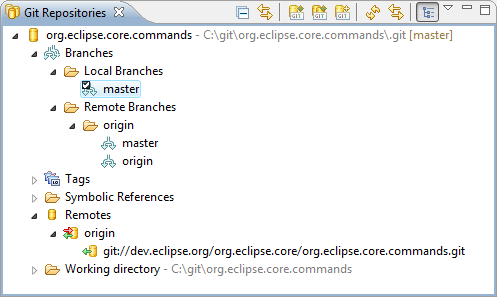
\includegraphics[width=8.4cm]{pics/EGit.png}    % The printed column width is 8.4 cm.
\caption{git repositories presented by EGit / JGit in Eclipse IDE \newline 
screenshot provided by http://eclipse.org/egit/ [2012-01-29]} 
\label{fig:JGit}
\end{center}
\end{figure}

Besides different, mostly platform dependent tools, 
SmartGit represents a current and functional GUI, which
is available on all popular operating system. Although SmartGit is sold commercially,
a free version for non-commercial usage is offered.




\subsection{git init \& clone}
At this point the local git repository can be set up by invoking the
command line command \textit{\lstinline!git init!} inside
the folder of the current project. The \textit{\lstinline!git clone!} 
command can be used for creating an exact copy of an available remote repository.

How to clone (copy) the source of this paper, including the entire changelog, to a local folder 
and thereby create a local repository as an exact replica of the online version,
is shown in \verb|line 1| of \textit{Listing \ref{git:clone}}. After the download has
finished, the document can be compiled using the provided \textit{run.sh} script. 

Note that the example in \textit{Listing \ref{git:clone}} shows how to compile 
the \LaTeX-file generated by R and Sweave (both are described in chapter \ref{sec:structure}).
Be aware that some settings need to be adapted to the local system. They are all stored
in \textit{./include/init.Rnw}. It is possible to maintain a local configuration and 
merge updates with the local source code by removing this file from the repository.
It is also necessary to install all loaded R packages (\textit{install.packages('name')}).

There is a script (\textit{run.sh}) included which helps creating the document.

Although the implementation of the sources takes place on
Linux distributions, the compilation should flawlessly work on other operating systems (OS) too.
While the tools themselves are used in the same way on all popular systems, some details
- like changing the directory using a terminal and setting up the search path to the binaries - is sometimes different.
If the creation of the PDF-file does not work on a specific setup, a prefabricated
version is also located in the git repository. 

\lstset{language=bash,caption={Clone git repository of this paper and compile the included \LaTeX-file},label=git:clone,
	morekeywords={git,cd,pdflatex,bibtex}}
\begin{lstlisting}
git clone git://github.com/FlorianEndel/Mathmod2012.git
cd Mathmod2012

# start R & Sweave
R CMD Sweave Mathmod2012_R_Geospatial_Plotting.Rnw

# if there was no error...
pdflatex Mathmod2012_R_Geospatial_Plotting.tex

# Bibtex for References
bibtex Mathmod2012_R_Geospatial_Plotting

# 2x pdflatex to get all indices right
pdflatex Mathmod2012_R_Geospatial_Plotting.tex
pdflatex Mathmod2012_R_Geospatial_Plotting.tex

# shellscript executing this tasks
./run.sh
\end{lstlisting}

After creating a new local git repository or cloning remote sources, everyting is ready for
editing the contents. Git does not anticipate specific software tools like special editors or file browsers. Any file in 
the repository can be edited using any favorite program. Solely the folder (including all contents)
\textit{.git} has to remain untouched. Otherwise the local repository can easily be damaged.

\subsection{git commit, pull, push}
All changes can be permanently 
added to git's history (the changelog) using \textit{\lstinline!git commit!} followed by a 
summary of the changes made (line 1 in listing \ref{git:pullpush_simple}). 
A committed version of the whole project can be restored later on and users are able to
track all changes over time. This is useful in case something breaks during 
the implementation of a new feature or adjustment of existing code.
Also try and error approaches may be applied, because resetting a previous state of the entire project is 
rather easy and fast. If an elder version of the project is required, for example to compare 
published and updated versions or include comments from a review process, activating  
a previous commit using \textit{\lstinline!git checkout [commit-id]!} is feasible.

After committing changes to the \textit{local} repository, it is possible to merge the local version 
with the remote repository (if any exists and is configured) and show all alterations to other team members or a
public audience. Before someone pushes the local version to a (central) git server, all changes made
by other people have to be downloaded and included into the own \textit{branch} of the project's source.
Downloading and merging can easily be carried out using \textit{\lstinline!git fetch!} and 
\textit{\lstinline!git merge!}. The command \textit{\lstinline!git pull!} is a combination of
these two steps.

If the remote and the local version do not contain any conflicting changes, 
git should be able to merge everything on its own flawlessly. However, sooner or later every team
faces the problem of conflicting and failing merges. Unfortunately the solution for such issues is not straight forward.
Because the official documentation of git (\url{http://git-scm.com/documentation}) and a quick 
Internet search provides a variety of helpful procedures, 
there is no further explanation provided within this paper.

Especially for manual merging of conflicting source files a graphical interface may be very helpful.

Right after the (automatic or manual) merging is finished, it is highly recommended to compile 
the Sweave and \LaTeX-file once again to be sure that no new errors were introduced. When the merging and
testing procedure is successfully finished, the local changes can be transfered to another remote repository
using \textit{\lstinline!git push!}.

As uploading (pushing) requires the right to write on a remote location, more configuration is usually 
necessary. There are several possibilities to authenticate to a remote location, 
including some additional tools, signation and encryption. Therefore no general explanation can be provided.

The source of this paper is hosted by the free (git) provider \url{github.com}. As shown in 
Listing \ref{git:clone}, it is quite easy to copy (clone) a project from their web-servers. 
Uploading (pushing) needs some extra configuration which is explained in the excellent tutorial
provided on \url{help.github.com} (pushing: \url{help.github.com/remotes/#pushing}).

\lstset{language=bash,caption={pull and push of a local git repository without merge conflicts},label=git:pullpush_simple,
	morekeywords={git,cd,pdflatex}}
\begin{lstlisting}
git commit -m 'Summary of changes made'
git pull
./run.sh
# everything alright?
git push
\end{lstlisting}

\subsection{git: further features}
There are much more useful features of git, waiting to be explored and used. Yet again
official documentation on \url{http://git-scm.com/documentation} and practical
tutorials, for example from \url{help.github.com}, are recommended.

In the following listing the most important 'advanced' features are summarized
(in alphabetical order):
\begin{description}
\item [add] \textit{\lstinline!git add!} is used to add newly created files (within the  folder managed by git) to the current repository.
\item [{branch}] Different branches of the same code-base can be edited independently from
another. In fact, every local clone of a remote repository represents a (remote tracking) 
branch. Branches may be combined using \textit{merge}.
\item [checkout] Switching between different branches (and even create new branches) can
be established using \textit{\lstinline!git checkout!}. Even previously committed versions
can be activated.
\item [log] Using the command \textit{\lstinline!git log!} all previous commit messages of
the currently activated branch are shown.
\item [{rebase}] allows to easily change a series of commits, reordering, editing, or squashing commits together into a single one. 
It is highly recommended that manipulating the history is performed with great care, because this is one of the 
rare possibilities to actually loose changes or (under special circumstances) even destroy the repository.
\item [reset] The \textit{\lstinline!git reset!} command is one of the most complicated
functions of git. Be aware that using \textit{reset} may delete data
irretrievably! Reseting files or complete (committed) versions
of a branch, mixing different versions and revoking committed files are some areas of application. 
A deeper understanding of git's different states -
unstaged, staged, committed - is necessary to effectively use \textit{reset}. A short
and informative introduction to the 'normal workflow' of git can be found here: \url{http://learn.github.com/p/normal.html}.
\item [status] \textit{\lstinline!git status!} shows the status of
the currently activated branch. Most notably new and changed files which may be involved
in the next commit are listed.
\item [tag] is a special label applied to a specific commit. For example a specific revision
of this paper's repository is marked (tagged) as published.
\end{description}


\begin{figure}[h]
\begin{center}
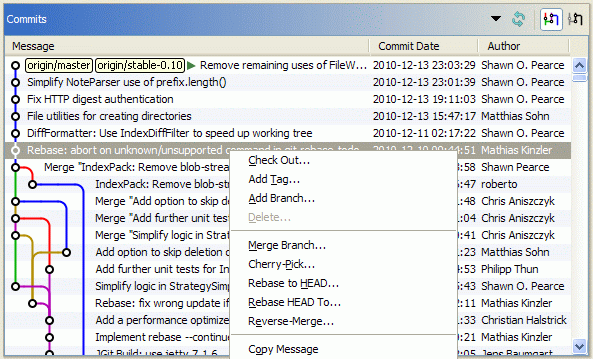
\includegraphics[width=8.4cm]{pics/Smartgit_graphical_Log.png}    % The printed column width is 8.4 cm.
\caption{example for a git changelog and history of commits visualized with Smartgit \newline 
screenshot provided by http://www.syntevo.com/smartgit [2012-01-29]} 
\label{fig:gitHistory}
\end{center}
\end{figure}

\section{\LaTeX, R \& Sweave}\label{sec:structure}

Once the git repository is set up, the Sweave document has to be arranged. 
In the following paragraphs involved technologies are briefly introduced.

Some essential properties are shared by all of them. Availability under an open source license, 
platform independence, multilingualism, extensive documentation and a strong proven 
community willing to help are the most important characteristics of these products.


\subsection{R}
R \citep{R} is known as an upcoming statistical environment. 

As an open source successor of S, it is known to be a powerful and flexible programming language
and computing environment. Especially everyones ability to utilize and
contribute to the very rich environment of additional packages hosted 
mainly on “The Comprehensive R Archive Network” are good reasons to give R a try. 
More advanced userRs (spelling “user” and “developer” with capital
’R’s is common in the R community) may use different extensions in 
addition to the variety of basic packages a basic installation offers.
Most packages provide worthwhile introductions and there even is special literature
for some of them.

R is mainly used via a command line interface. Although this - in comparison
to current graphical user interfaces outdated - way to communicate 
with a computer program got a quite steep learning curve, the practical 
advantages are convicting many users to stick with it. Mainly the
ease of combining playful exploration of datasets and automatic
reproduction of any steps taken, using script- or batch-files, are advantageous.

Also the following examples, using special packages providing methods 
for spatial data, may be executed on a simple terminal, a graphical front-end to R,
a remote server or within a Sweave document. This flexibility enables 
the usage of the same R source code within a database
\footnote{for example \textit{plr} (\url{http://www.joeconway.com/plr/} [2012-01-30]) for PostgreSQL 
\citep{group2011postgresql}}, a local PC and even servers and cloud services.

Of course there also are some graphical user interfaces, which may support
the usage of R. The most popular and beginner friendly solutions are
Eclipse with the StatEt extension and the recently published RStudio
(\url{http://rstudio.org/}). Both are open source and platform independent solution,
which offer lots of advantages like project management, integration of version 
management (git), support for Sweave and a client/server separation.

While Eclipse provides considerably more additional plugins and possibilities,
RStudio can be highly recommended to all useRs.

\subsection{Sweave}
In the official manual \citep{Sweave:Leisch:2002} Sweave is defined as follows:
\begin{quotation}
Sweave provides a flexible 
framework for mixing text 
and S code for automatic document generation. 
A single source file contains both documentation text and S code, which are then woven
into a final document
\end{quotation} 

As explained before, R is an open source implementation of S.

In 2002, Sweave was presented in the former "R Journal"
(\url{http://journal.r-project.org/}) called "R News" (official archive of R News: \url{http://cran.r-project.org/doc/Rnews/}). In the first part of this 
introduction, Sweave is described briefly \citep{Sweave:Leisch:2002}:

\begin{quotation}
The purpose of Sweave is to create dynamic reports, 
which can be updated automatically if data or
analysis change. Instead of inserting a prefabricated
graph or table into the report, the master document
contains the R code necessary to obtain it. When run
through R, all data analysis output (tables, graphs, ...) 
is created on the fly and inserted into a final \LaTeX{}
document. The report can be automatically updated
if data or analysis change, which allows for truly reproducible research.
\end{quotation}

Usually Sweave files got the file extension \texttt{.Rnw}. 
After executing \texttt{R CMD Sweave} followed by the filename
of the Sweave document, all R-code is extracted from the document and executed using R.
The results are merged with the \LaTeX{} code of the \texttt{.Rnw} file and saved
as \texttt{.tex} file with the same filename. Afterwards the common 
compilation using \texttt{latex}, \texttt{pdflatex}, \texttt{bibtex}, and relatives
can be performed.

\subsection{simple Sweave document}

This subsection shows the basic structure of a Sweave document. As this
paper is written using \LaTeX{} and R, another working example can be found
in the git repository, described in Listing \ref{git:clone} on page
\pageref{git:clone}.

At the beginning (line 1 to 5) of Listing \ref{sweave:simple}, a very simple
\LaTeX-Document is shown. In line 6 an R-environment is declared using 
the "noweb" syntax \citep{Ramsey_1994, Johnson_Johnson_2000}.
Between \newline \texttt{<<label1, echo=false, results=hide>>=} \newline and the
"at"-sign, R source code can be located. The header of the environment holds
some (local) settings an the name, which is displayed during the
compilation process. The \textit{results} setting defines how
output generated by R should be handled by the \LaTeX{} processor and \textit{echo}
configures whether messages from R should be included in the output.

More details about configuration of the noweb-environment of Sweave can
be found in the official manual \citep{SweaveManual}.

Some additional functionalities are shown in the example. The content of
\texttt{\textbackslash{}Sexpr\{\#R-Code\}}
is also executed by R and any output is included in the document. This can be
useful when single values (of a calculation) are being inserted into continuous text.

\texttt{\textbackslash{}SweaveInput\{filename\}} can be used to include 
another Sweave file. Although importing additional source code can be realized with
R, partitioning a document into several Sweave files is advisable.

All single R environments which are executed within the same process share one
global namespace. Also libraries, like \texttt{xtable} (loaded on line 7), which eases the
creation of \LaTeX-tables out of data stored in R, are
available throughout the document.

\lstset{language=Octave,caption={basic structure of a Sweave document},label=sweave:simple}
\begin{lstlisting}
\documentclass[a4paper]{article}
% additional \LaTeX configuration

\begin{document}

<<label1, echo=false, results=hide>>=
library(xtable)
# R code following
@

<<LaTex_Output, echo=hide, results=tex>>=
# R code generating \LaTeX
@

<<>>=
# empty header, standard settings
@

Normal \LaTeX code and a single line from \Sexpr{print('R')}.

\SweaveInput{./includes/config}


\end{document}
\end{lstlisting} 



\section{geospatial plotting}

Finally, as the most important preparations are finished, some geospatial plots 
generated by R can be shown. In this document, a slightly more complex
setup for Sweave is used. 

Most current packages which are dealing with spatial data are using the
extensive \textit{sp} package \citep{RSpatialDataAnalysis}. Additionally
other extensions like \textit{maptools} to handle shapefiles, \textit{rgdal}
as bridge to the geospatial abstraction library "GDAL" (\url{http://www.gdal.org/})
and \textit{ggplot2} \citep{Rggplot2} for advanced graphics are used.

The connection to databases (PostgreSQL), usage of multiple processors 
in parallel (with \textit{snow} and \textit{snowfall} \citep{Rsnow, Rsnowfall}), 
advanced logging (\textit{log4r} \citep{Rlog4r}) and caching (\textit{cacheSweave}) 
are configured and partly used, but not explained in more detail.

\subsection{visualizing friendships of facebook users}
The first example is not created by the author. It illustrates not only a
beautiful graphic made with the help of R, but also caused
public interest and many speculations, whether such picture can be
created using an open source technology. (In fact R was used for plotting,
but some reworking took place afterwards.) The map shows the relation of 
facebook friends \citep{FacebookFriendMap}.

\begin{figure}[h]
\begin{center}
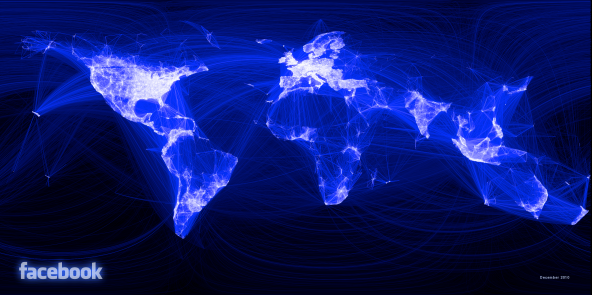
\includegraphics[width=8.4cm]{pics/facebook.png}    % The printed column width is 8.4 cm.
\caption{visualizing friendships of facebook users} 
\label{fig:facebook}
\end{center}
\end{figure}

\subsection{map connections with great circles}
After the mentioned discussion about the friendship plot of facebook users,
Nathan Yau of \url{flowingdata.com} showed how to use great circles
(Riemannian circle) provided by the \textit{geosphere} package. As an example he chose to
visualize flight data of US 
airports\footnote{\url{http://flowingdata.com/2011/05/11/how-to-map-connections-with-great-circles/}}.

The presented plot is an adoption of this work. Open Data sources are downloaded from
the Internet, combined and plotted within R and directly added to this document.
Therefore, changing the displayed airline or plotting more than one (in parallel using
multiple processors simultaneously), can be easily achieved.


\begin{figure}[h]
\begin{center}
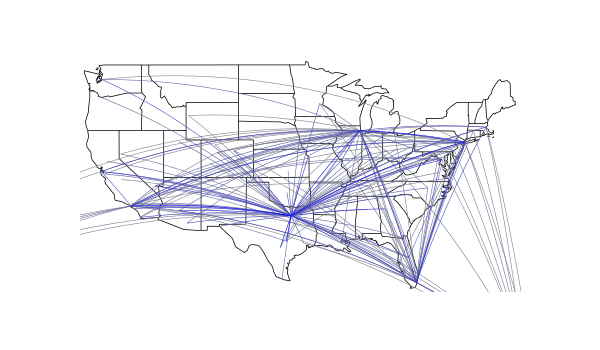
\includegraphics[width=8.4cm]{pics/flights.png}    % The printed column width is 8.4 cm.
\caption{flights of an US American airline in North America} 
\label{fig:flights}
\end{center}
\end{figure}

\subsection{Google Earth and Open Street Map}
Using the \textit{RgoogleMaps} package \citep{RgoogleMaps}, spatial data and
pictures provided by Google can be downloaded. To get access to the 
"Maps Image APIs" of Google a special key is necessary. Although limited access would be free
of charge, the provided example uses data from the OpenStreetMap project 
(\url{http://www.openstreetmap.org/}).

The package \textit{osmar 1.1-0} is specialized on the connection
between R and OpenStreetMap, but was (at least at Debian Sid) quite hard to install
and did not function correctly.

A map of Vienna and the surrounding region, which was loaded directly
from OpenStreetMap using R, is displayed in the following example. 
Also the manipulation of the map using coordinates is presented by marking
Vienna University of Technology (TU Vienna).


\begin{figure}[h]
\begin{center}
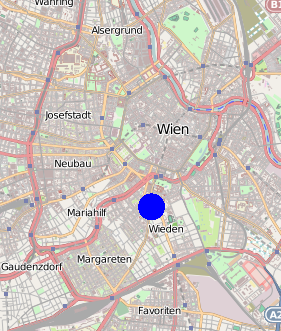
\includegraphics[width=7cm, angle=90]{pics/hometu.png}    % The printed column width is 8.4 cm.
\caption{manipulated OpenStreetMap of Vienna} 
\label{fig:hometu}
\end{center}
\end{figure}


\subsection{gadm.org}
The last example features a political map from 
the "GADM database of Global Administrative Areas" (\url{http://www.gadm.org/}).
Maps in different granularity and formats are provided (for academic or
non-profit reasons!) for free.

After loading the file with R, some corrections of the text encoding have
to be performed. The data seems to be stored as "UTF-8", but wrongly
imported and displayed in the "ISO-8859-2" format. After explicit conversion
everything should run smoothly.

To show the possibilities of this map, some federal states are removed. 
The coloring is created using a random heat-map. Only one region ("Tulln")
is completely black. Additionally all borders are painted black and the name
of each district is displayed over the particular centroid (without collisions).



\section{result}
These simple examples 
may induce a vision  of the vast possibilities the presented techniques, and 
especially their combination, offer. Integration with established systems like Grass,
utilization of Open Data and Open Government resources, cloud computing and many other 
current trends can all be handled. The low price and
freedom open source software provides is just another reason to try out
these modern programs.

Summarizing not only the spatial plots themselves, but also the entire workflow
of a (distributed) project using Git, Sweave, R and LaTeX is the result and 
message of this paper.



\begin{figure}[h]
\begin{center}
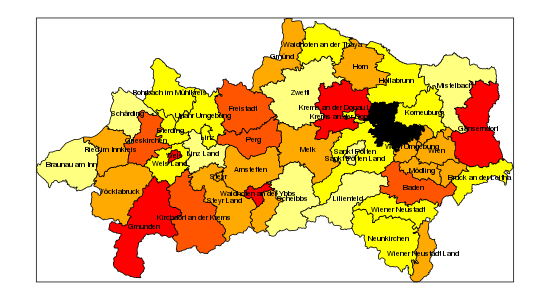
\includegraphics[width=10cm]{pics/northAustria.png}    % The printed column width is 8.4 cm.
\caption{lower Austria from gadm.org} 
\label{fig:noe}
\end{center}
\end{figure}

\bibliography{lit}   

\end{document}
